
\chapter{Wyniki dla pozostałych maszyn wirtualnych}

\begin{table}[p]
	\begin{center}        
 		\begin{tabular}{l r r r r } \toprule
 & \emph{bpr} & \emph{divsufsort} & \emph{qsufsort} & \emph{skew}\\ \midrule
\texttt{abac} & 1.83 & 0.05 & \textbf{0.03} & 0.06\\
\texttt{abba} & 4.41 & \textbf{2.82} & 2.85 & 11.62\\
\texttt{book1x20} & \textbf{3.85} & 4.36 & 4.24 & 23.35\\
\texttt{fib\_s14930352} & 11.77 & 6.18 & \textbf{4.15} & 15.18\\
\texttt{fss10} & 6.50 & 4.87 & \textbf{3.04} & 12.26\\
\texttt{fss9} & 1.31 & 0.80 & \textbf{0.69} & 2.32\\
\texttt{houston} & 4.05 & \textbf{0.23} & 0.53 & 1.45\\
\texttt{paper5x80} & 0.19 & 0.15 & \textbf{0.07} & 0.53\\
\texttt{test1} & 3.14 & 0.49 & \textbf{0.25} & 2.27\\
\texttt{test2} & 0.96 & 0.36 & \textbf{0.23} & 2.28\\
\texttt{test3} & 88.37 & 0.54 & \textbf{0.42} & 1.22\\
 \midrule
Total & 126.39 & 20.85 & \textbf{16.51} & 72.53\\
 \bottomrule
\end{tabular}

    \end{center}                         
	\caption{Czas działania algorytmów na plikach z korpusu \texttt{The Gauntlet} dla maszyny wirtualnej \texttt{ibm}.}%
    \label{tab:ibm-gauntlet}
\end{table}

\begin{figure}[p]
   \begin{center}
        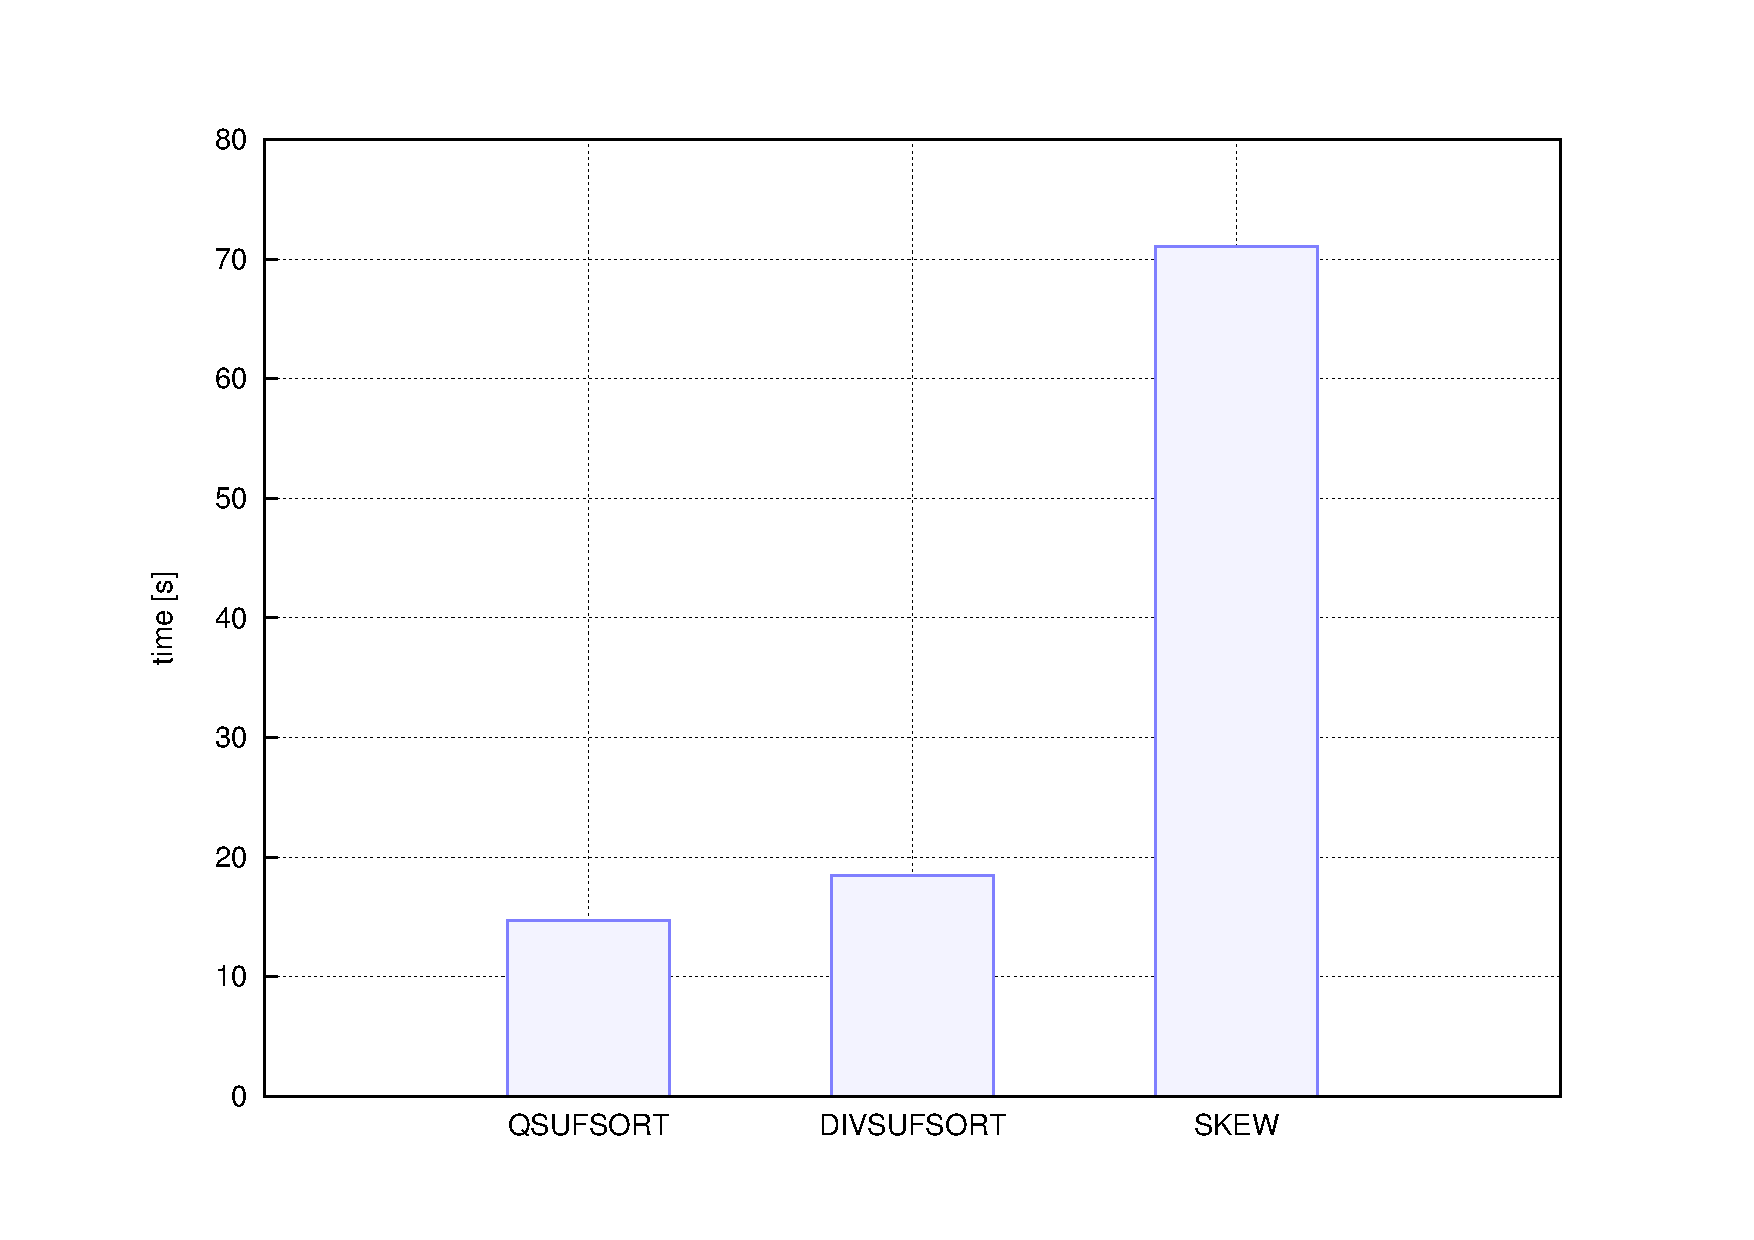
\includegraphics[width=\linewidth]{figures/results/ibm-gauntlet.pdf}
    \end{center}        
    \caption{Sumaryczny czas działania algorytmów na plikach z korpusu \texttt{The Gauntlet} dla maszyny wirtualnej \texttt{ibm}.}%
    \label{rys:ibm-gauntlet}
\end{figure}


\begin{table}[p]
	\begin{center}        
 		\begin{tabular}{l r r r r } \toprule
 & \emph{bpr} & \emph{divsufsort} & \emph{qsufsort} & \emph{skew}\\ \midrule
\texttt{chr22.dna} & \textbf{7.31} & 8.54 & 8.15 & 60.73\\
\texttt{etext99} & 28.21 & 29.20 & \textbf{26.35} & ---\\
\texttt{gcc-3.0.tar} & --- & 17.25 & \textbf{14.81} & ---\\
\texttt{howto} & 8.44 & 10.33 & \textbf{7.94} & 79.66\\
\texttt{jdk13c} & 16.44 & 14.74 & \textbf{12.36} & ---\\
\texttt{linux-2.4.5.tar} & 25.60 & 24.09 & \textbf{20.30} & ---\\
\texttt{rctail96} & 30.55 & 28.08 & \textbf{24.60} & ---\\
\texttt{rfc} & 28.93 & 25.92 & \textbf{24.43} & ---\\
\texttt{sprot34.dat} & 28.55 & 28.94 & \textbf{22.89} & ---\\
\texttt{w3c2} & 24.87 & 25.55 & \textbf{17.29} & ---\\
 \midrule
Total &  & 212.62 & \textbf{179.12} & \\
 \bottomrule
\end{tabular}
 
    \end{center}                         
	\caption{Czas działania algorytmów na plikach z korpusu Giovanniego Manziniego dla maszyny wirtualnej \texttt{ibm}.}%
    \label{tab:ibm-manzini}
\end{table}

\begin{figure}[p]
       \begin{center}
            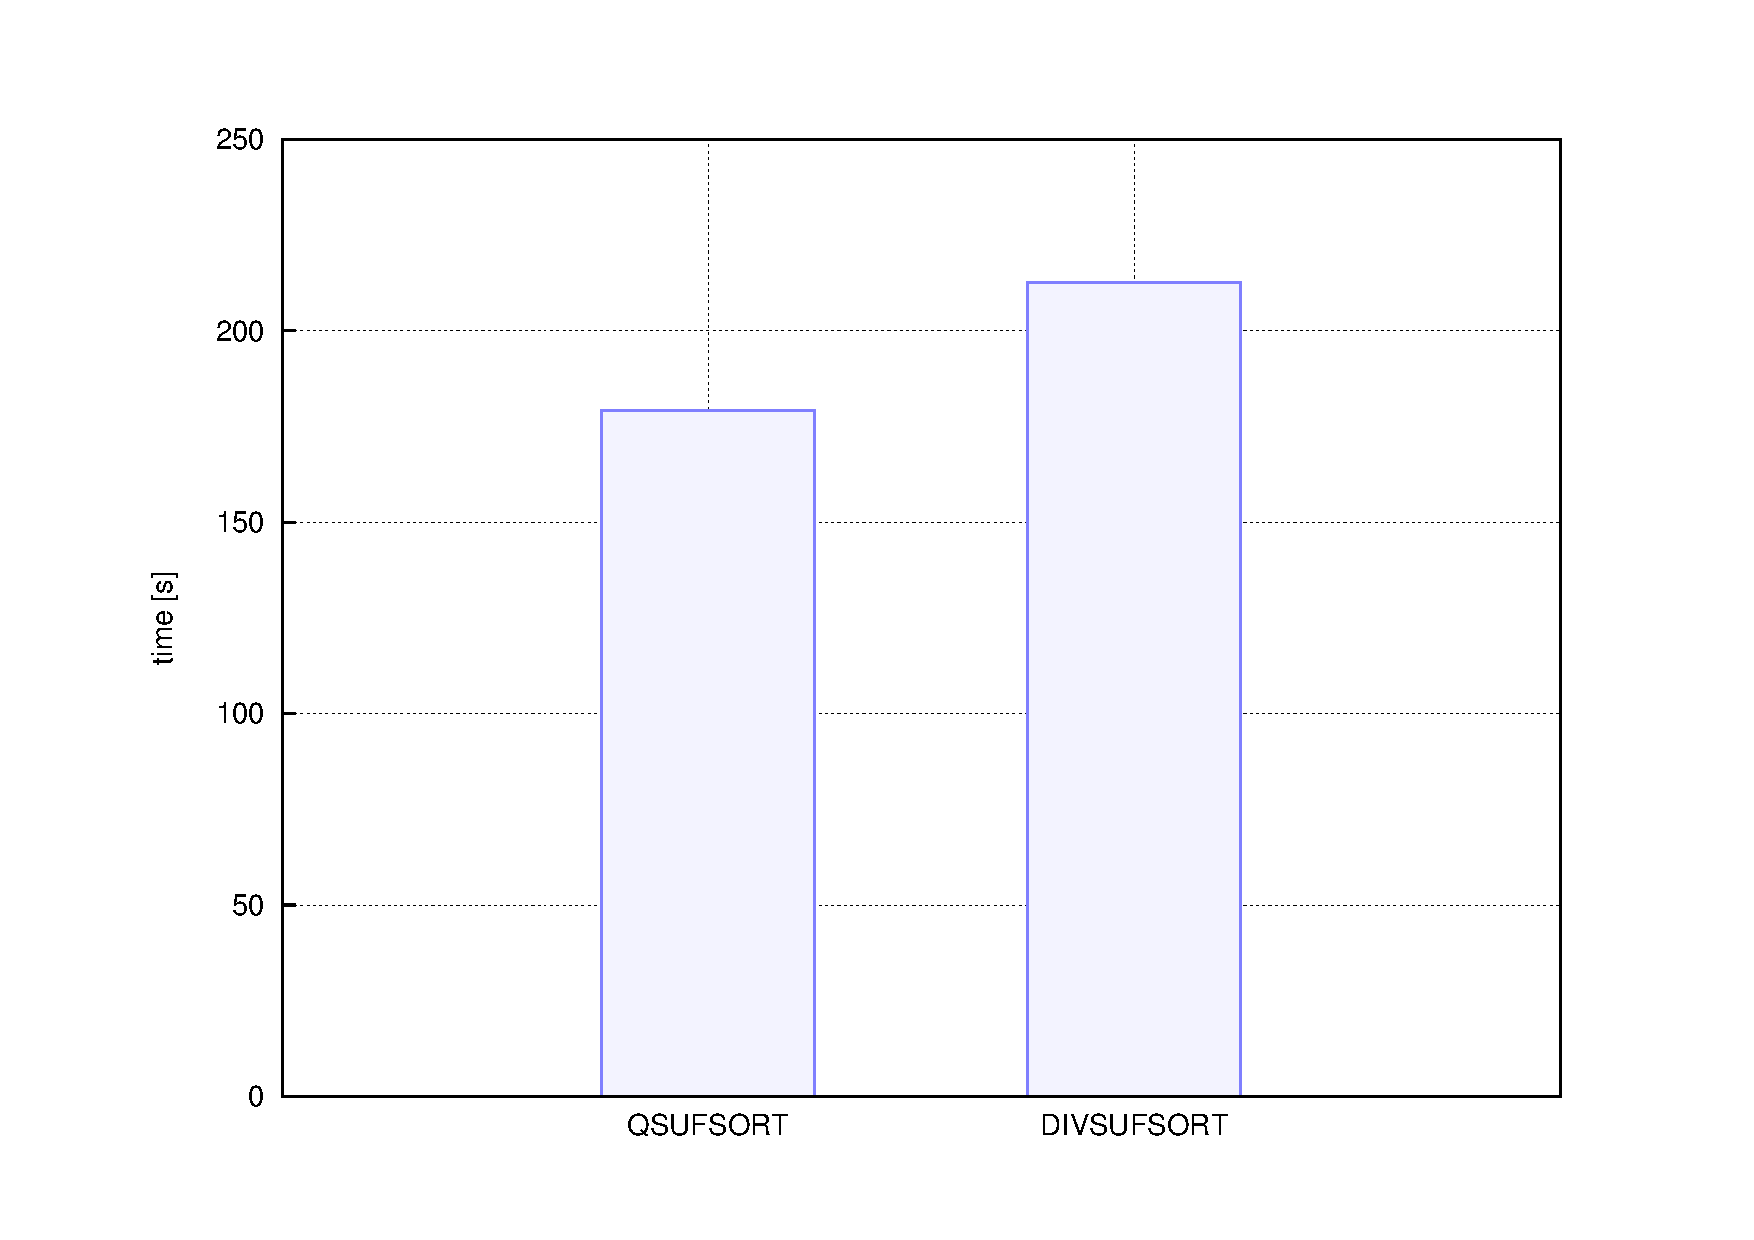
\includegraphics[width=\linewidth]{figures/results/ibm-manzini.pdf}
        \end{center}        
	    \caption{Sumaryczny czas działania algorytmów na plikach z korpusu Giovanniego Manziniego dla maszyny wirtualnej \texttt{ibm}.}%
    \label{rys:ibm-manzini}
\end{figure}
 

\begin{table}[p]
	\begin{center}        
 		\begin{tabular}{l r r r r } \toprule
 & \emph{bpr} & \emph{divsufsort} & \emph{qsufsort} & \emph{skew}\\ \midrule
\texttt{abac} & 1.83 & 0.05 & \textbf{0.03} & 0.06\\
\texttt{abba} & 4.41 & \textbf{2.82} & 2.85 & 11.62\\
\texttt{book1x20} & \textbf{3.85} & 4.36 & 4.24 & 23.35\\
\texttt{fib\_s14930352} & 11.77 & 6.18 & \textbf{4.15} & 15.18\\
\texttt{fss10} & 6.50 & 4.87 & \textbf{3.04} & 12.26\\
\texttt{fss9} & 1.31 & 0.80 & \textbf{0.69} & 2.32\\
\texttt{houston} & 4.05 & \textbf{0.23} & 0.53 & 1.45\\
\texttt{paper5x80} & 0.19 & 0.15 & \textbf{0.07} & 0.53\\
\texttt{test1} & 3.14 & 0.49 & \textbf{0.25} & 2.27\\
\texttt{test2} & 0.96 & 0.36 & \textbf{0.23} & 2.28\\
\texttt{test3} & 88.37 & 0.54 & \textbf{0.42} & 1.22\\
 \midrule
Total & 126.39 & 20.85 & \textbf{16.51} & 72.53\\
 \bottomrule
\end{tabular}

    \end{center}                         
	\caption{Czas działania algorytmów na plikach z korpusu \texttt{The Gauntlet} dla maszyny wirtualnej \texttt{jrockit}.}%
    \label{tab:jrockit-gauntlet}
\end{table}

\begin{figure}[p]
       \begin{center}
            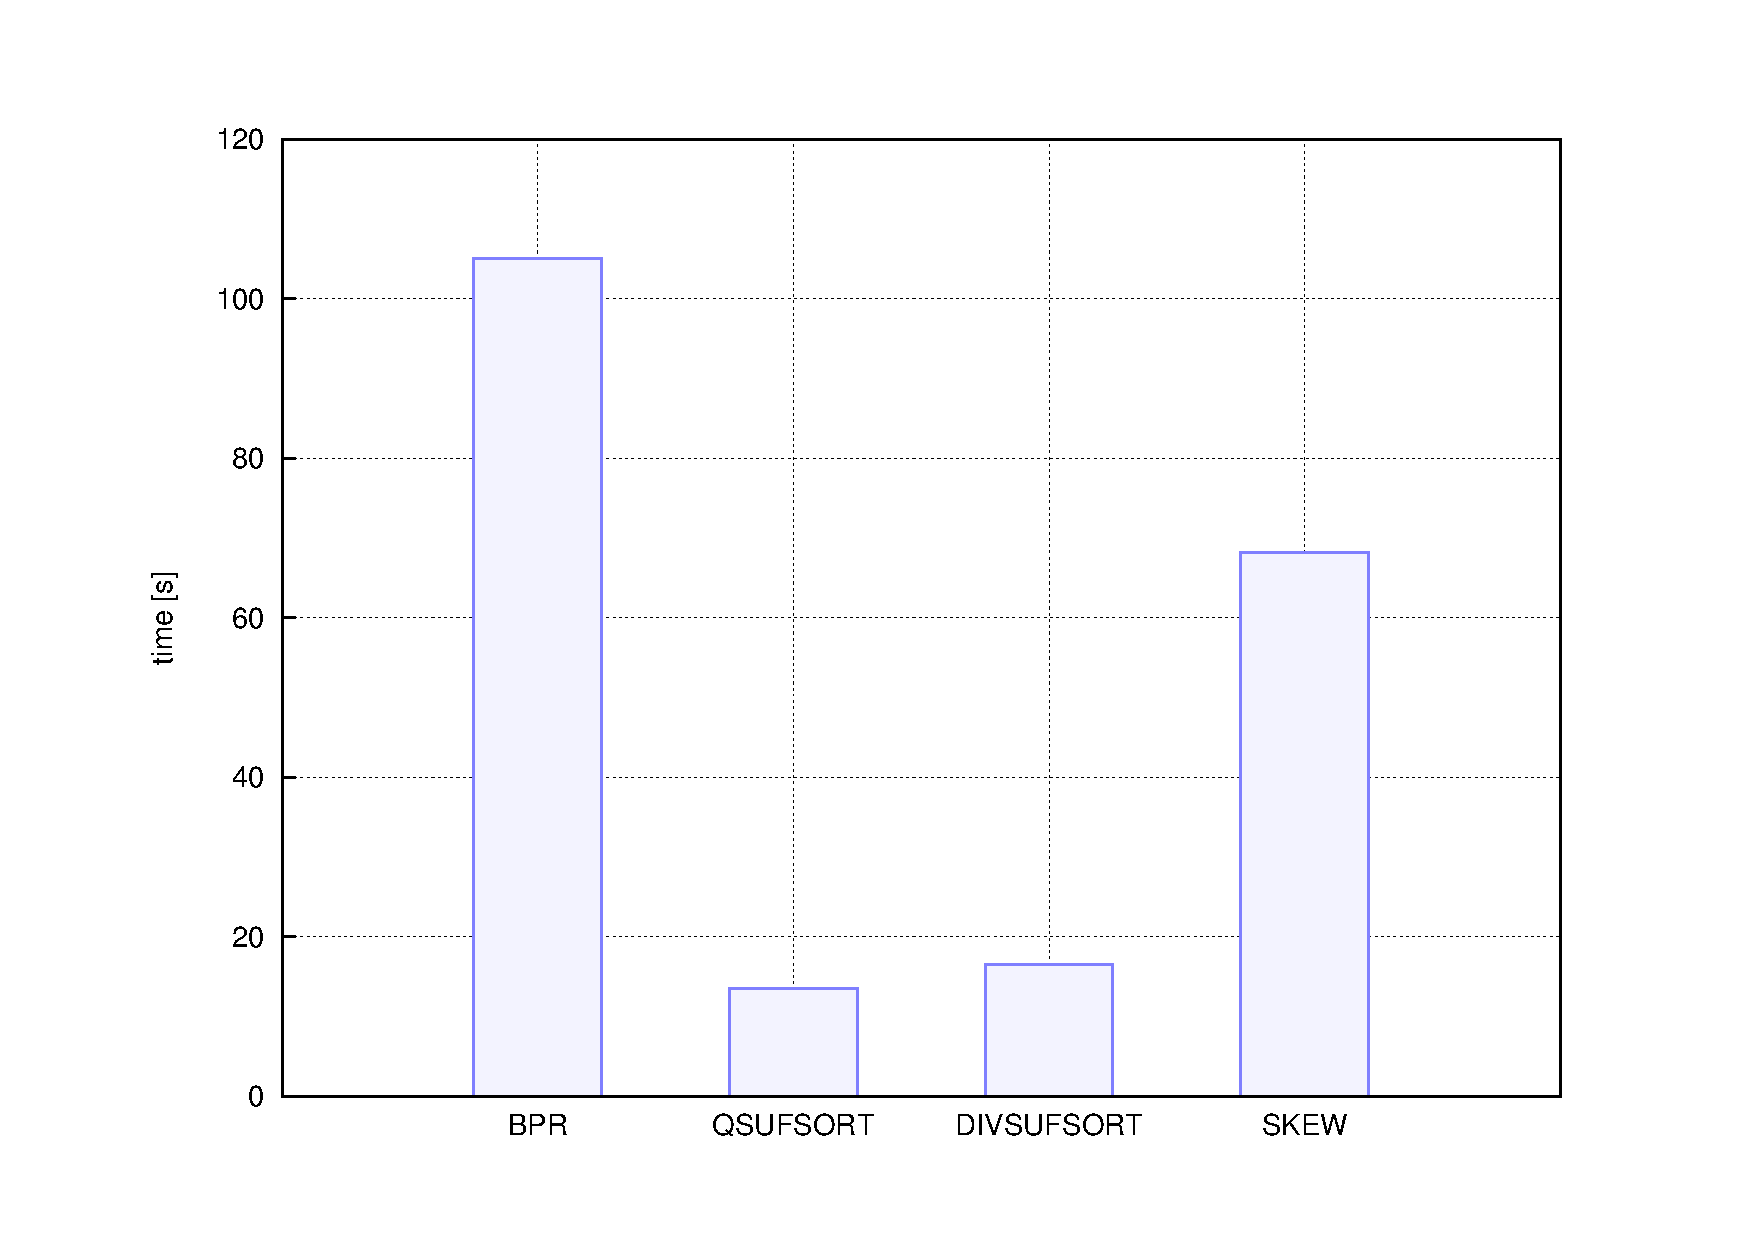
\includegraphics[width=\linewidth]{figures/results/jrockit-gauntlet.pdf}
        \end{center}        
	    \caption{Sumaryczny czas działania algorytmów na plikach z korpusu \texttt{The Gauntlet} dla maszyny wirtualnej \texttt{jrockit}.}%
    \label{rys:jrockit-gauntlet}
\end{figure} 


\begin{table}[p]
	\begin{center}        
 		\begin{tabular}{l r r r r } \toprule
 & \emph{bpr} & \emph{divsufsort} & \emph{qsufsort} & \emph{skew}\\ \midrule
\texttt{chr22.dna} & \textbf{7.31} & 8.54 & 8.15 & 60.73\\
\texttt{etext99} & 28.21 & 29.20 & \textbf{26.35} & ---\\
\texttt{gcc-3.0.tar} & --- & 17.25 & \textbf{14.81} & ---\\
\texttt{howto} & 8.44 & 10.33 & \textbf{7.94} & 79.66\\
\texttt{jdk13c} & 16.44 & 14.74 & \textbf{12.36} & ---\\
\texttt{linux-2.4.5.tar} & 25.60 & 24.09 & \textbf{20.30} & ---\\
\texttt{rctail96} & 30.55 & 28.08 & \textbf{24.60} & ---\\
\texttt{rfc} & 28.93 & 25.92 & \textbf{24.43} & ---\\
\texttt{sprot34.dat} & 28.55 & 28.94 & \textbf{22.89} & ---\\
\texttt{w3c2} & 24.87 & 25.55 & \textbf{17.29} & ---\\
 \midrule
Total &  & 212.62 & \textbf{179.12} & \\
 \bottomrule
\end{tabular}
 
    \end{center}                         
\caption{Czas działania algorytmów na plikach z korpusu Giovanniego Manziniego dla maszyny wirtualnej \texttt{jrockit}.}%
    \label{tab:jrockit-manzini}
\end{table}

\begin{figure}[p]
       \begin{center}
            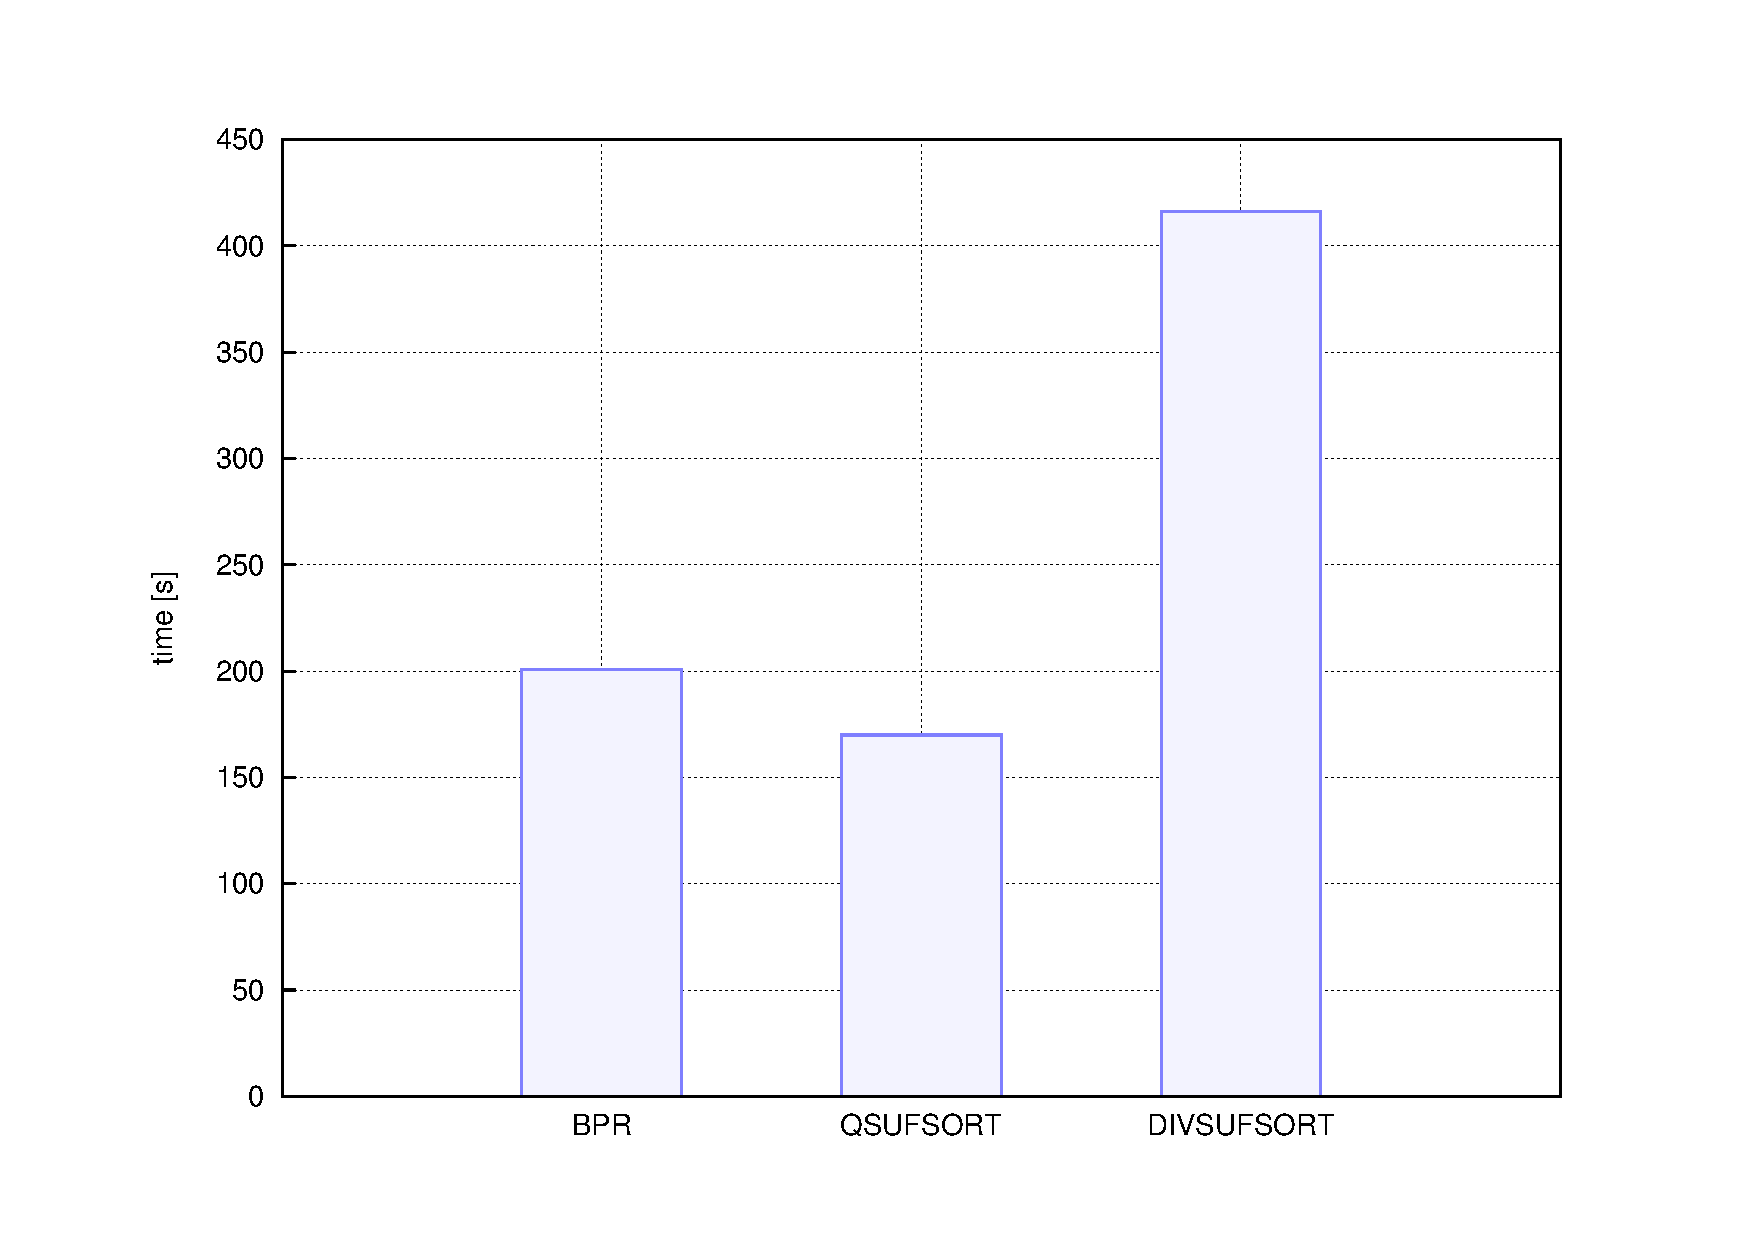
\includegraphics[width=\linewidth]{figures/results/jrockit-manzini.pdf}
        \end{center}        
	    \caption{Sumaryczny czas działania algorytmów na plikach z korpusu Giovanniego Manziniego dla maszyny wirtualnej \texttt{jrockit}.}%
    \label{rys:jrockit-manzini}
\end{figure} 


\begin{table}[p]
	\begin{center}        
 		\begin{tabular}{l r r r r } \toprule
 & \emph{bpr} & \emph{divsufsort} & \emph{qsufsort} & \emph{skew}\\ \midrule
\texttt{abac} & 1.83 & 0.05 & \textbf{0.03} & 0.06\\
\texttt{abba} & 4.41 & \textbf{2.82} & 2.85 & 11.62\\
\texttt{book1x20} & \textbf{3.85} & 4.36 & 4.24 & 23.35\\
\texttt{fib\_s14930352} & 11.77 & 6.18 & \textbf{4.15} & 15.18\\
\texttt{fss10} & 6.50 & 4.87 & \textbf{3.04} & 12.26\\
\texttt{fss9} & 1.31 & 0.80 & \textbf{0.69} & 2.32\\
\texttt{houston} & 4.05 & \textbf{0.23} & 0.53 & 1.45\\
\texttt{paper5x80} & 0.19 & 0.15 & \textbf{0.07} & 0.53\\
\texttt{test1} & 3.14 & 0.49 & \textbf{0.25} & 2.27\\
\texttt{test2} & 0.96 & 0.36 & \textbf{0.23} & 2.28\\
\texttt{test3} & 88.37 & 0.54 & \textbf{0.42} & 1.22\\
 \midrule
Total & 126.39 & 20.85 & \textbf{16.51} & 72.53\\
 \bottomrule
\end{tabular}

    \end{center}                         
	\caption{Czas działania algorytmów na plikach z korpusu \texttt{The Gauntlet} dla maszyny wirtualnej \texttt{harmony}.}%
    \label{tab:harmony-gauntlet}
\end{table}

\begin{figure}[p]
       \begin{center}
            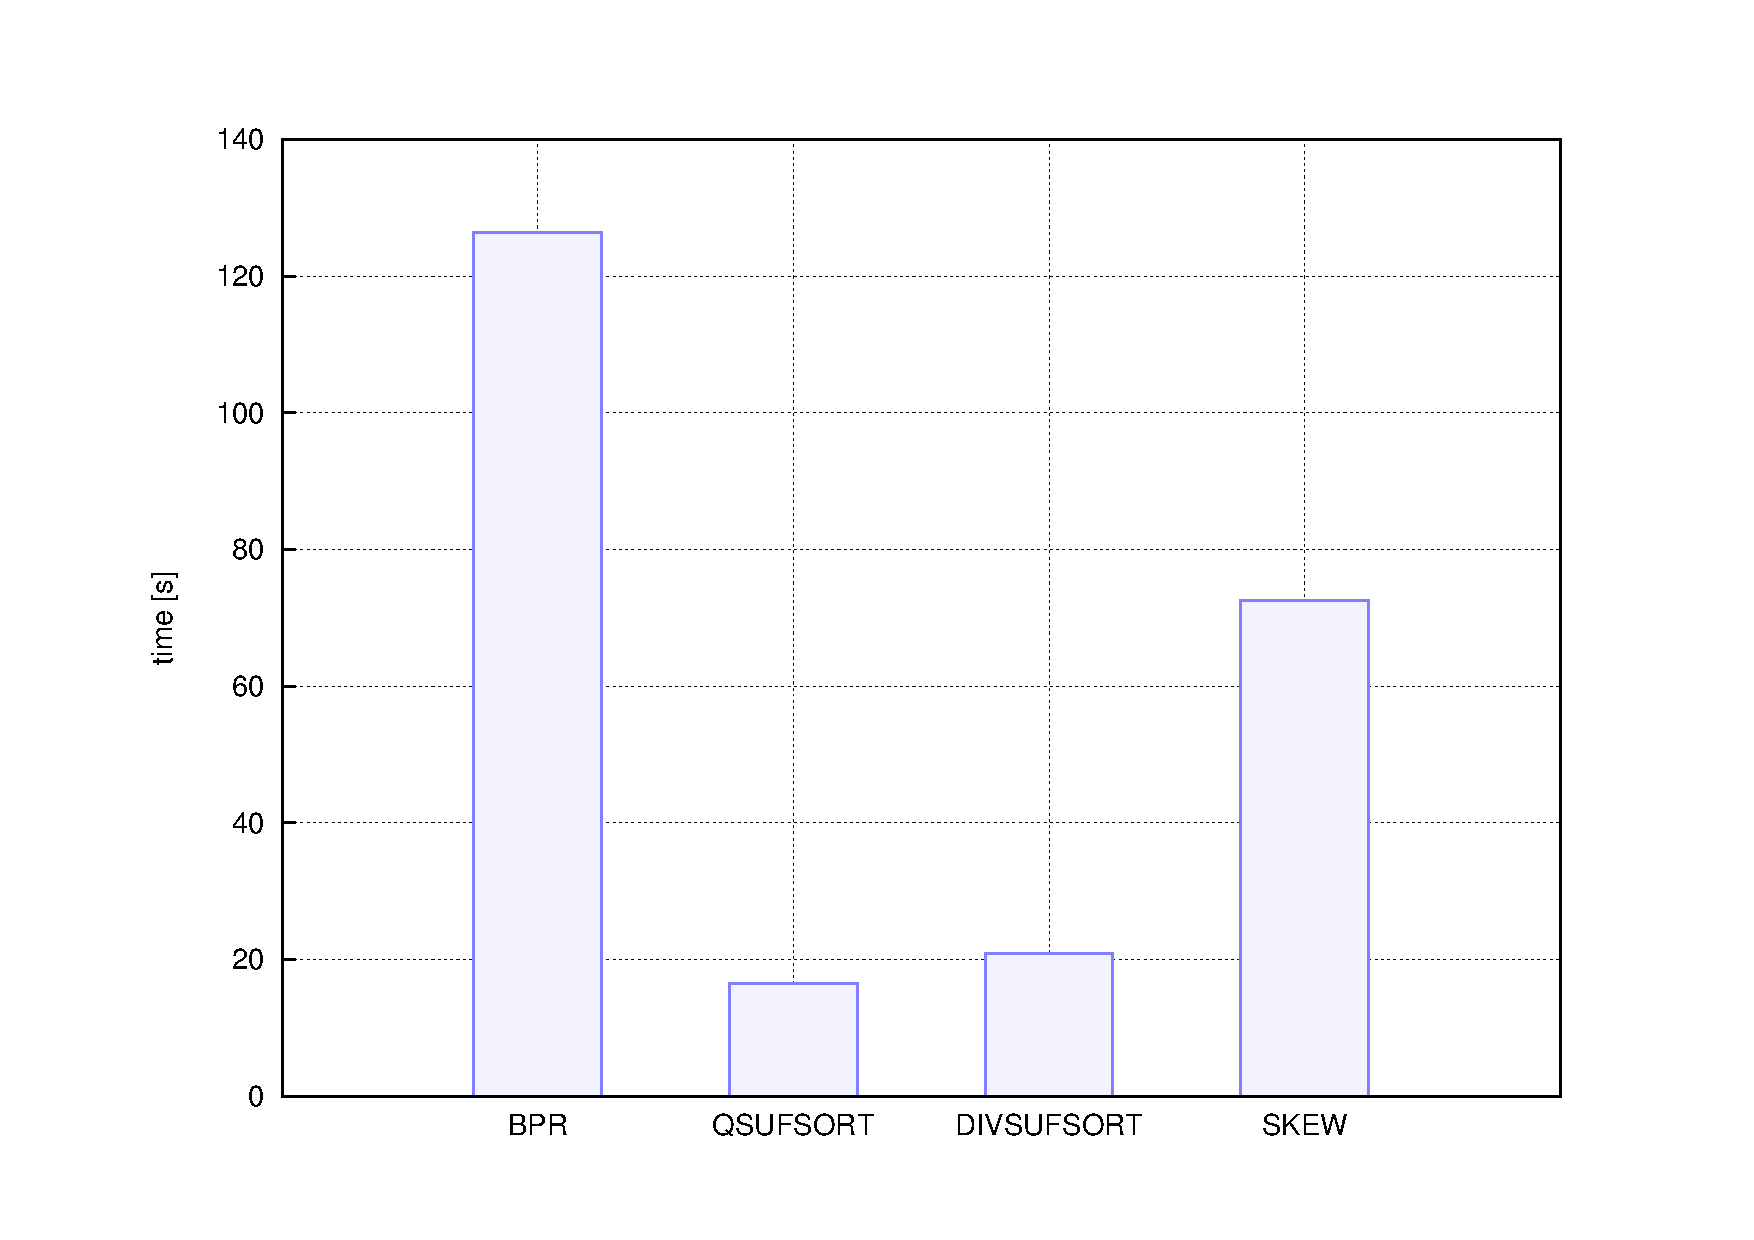
\includegraphics[width=\linewidth]{figures/results/harmony-gauntlet.pdf}
        \end{center}        
	    \caption{Sumaryczny czas działania algorytmów na plikach z korpusu \texttt{The Gauntlet} dla maszyny wirtualnej \texttt{harmony}.}%
    \label{rys:harmony-gauntlet}
\end{figure} 


\begin{table}[p]
	\begin{center}        
 		\begin{tabular}{l r r r r } \toprule
 & \emph{bpr} & \emph{divsufsort} & \emph{qsufsort} & \emph{skew}\\ \midrule
\texttt{chr22.dna} & \textbf{7.31} & 8.54 & 8.15 & 60.73\\
\texttt{etext99} & 28.21 & 29.20 & \textbf{26.35} & ---\\
\texttt{gcc-3.0.tar} & --- & 17.25 & \textbf{14.81} & ---\\
\texttt{howto} & 8.44 & 10.33 & \textbf{7.94} & 79.66\\
\texttt{jdk13c} & 16.44 & 14.74 & \textbf{12.36} & ---\\
\texttt{linux-2.4.5.tar} & 25.60 & 24.09 & \textbf{20.30} & ---\\
\texttt{rctail96} & 30.55 & 28.08 & \textbf{24.60} & ---\\
\texttt{rfc} & 28.93 & 25.92 & \textbf{24.43} & ---\\
\texttt{sprot34.dat} & 28.55 & 28.94 & \textbf{22.89} & ---\\
\texttt{w3c2} & 24.87 & 25.55 & \textbf{17.29} & ---\\
 \midrule
Total &  & 212.62 & \textbf{179.12} & \\
 \bottomrule
\end{tabular}
 
    \end{center}                         
	\caption{Czas działania algorytmów na plikach z korpusu Giovanniego Manziniego dla maszyny wirtualnej \texttt{harmony}.}%
    \label{tab:harmony-manzini}
\end{table}

\begin{figure}[p]
       \begin{center}
            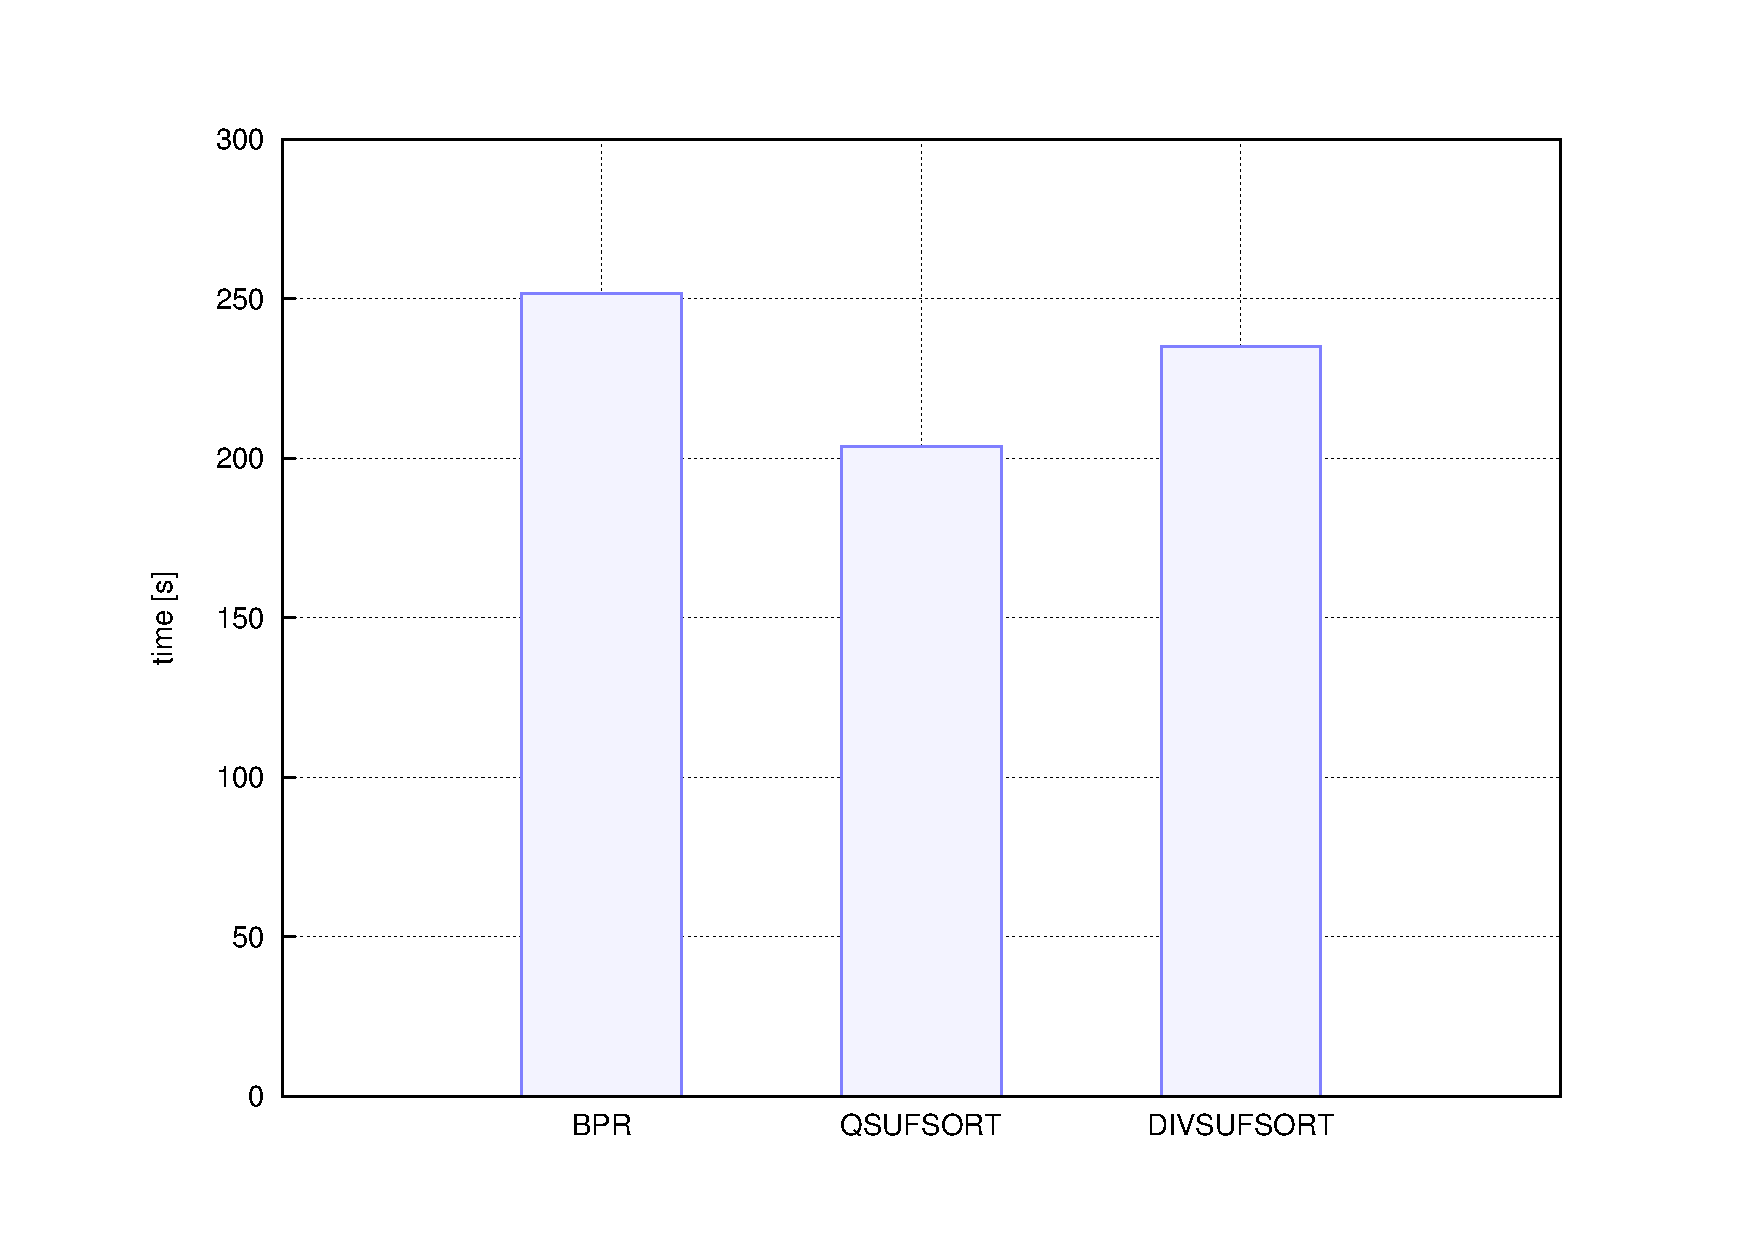
\includegraphics[width=\linewidth]{figures/results/harmony-manzini.pdf}
        \end{center}        
	    \caption{Sumaryczny czas działania algorytmów na plikach z korpusu Giovanniego Manziniego dla maszyny wirtualnej \texttt{harmony}.}%
    \label{rys:harmony-manzini}
\end{figure}
 